%=====================================================================
\section{Neural Nets}
%=====================================================================

\begin{frame}
	\frametitle{Outline}
	
	\begin{itemize}
		\item Understanding Neural Nets
		\item Practical Considerations
		\item Extended examples
	\end{itemize}
\end{frame}

\begin{frame}
	\frametitle{Neural Nets}
	\begin{itemize}
		\item Around since the 1950ies
		\item Underwent different development steps, e.g.
		\begin{itemize}
			\item use of backpropagation
			\item GPUs
		\end{itemize}
		\item Black Box
		\item TensorFlow/Keras, PyTorch
	\end{itemize}
\end{frame}

\begin{frame}
	\frametitle{``Swiss Army Knife'' among ML Algorithms}
	\begin{figure}
		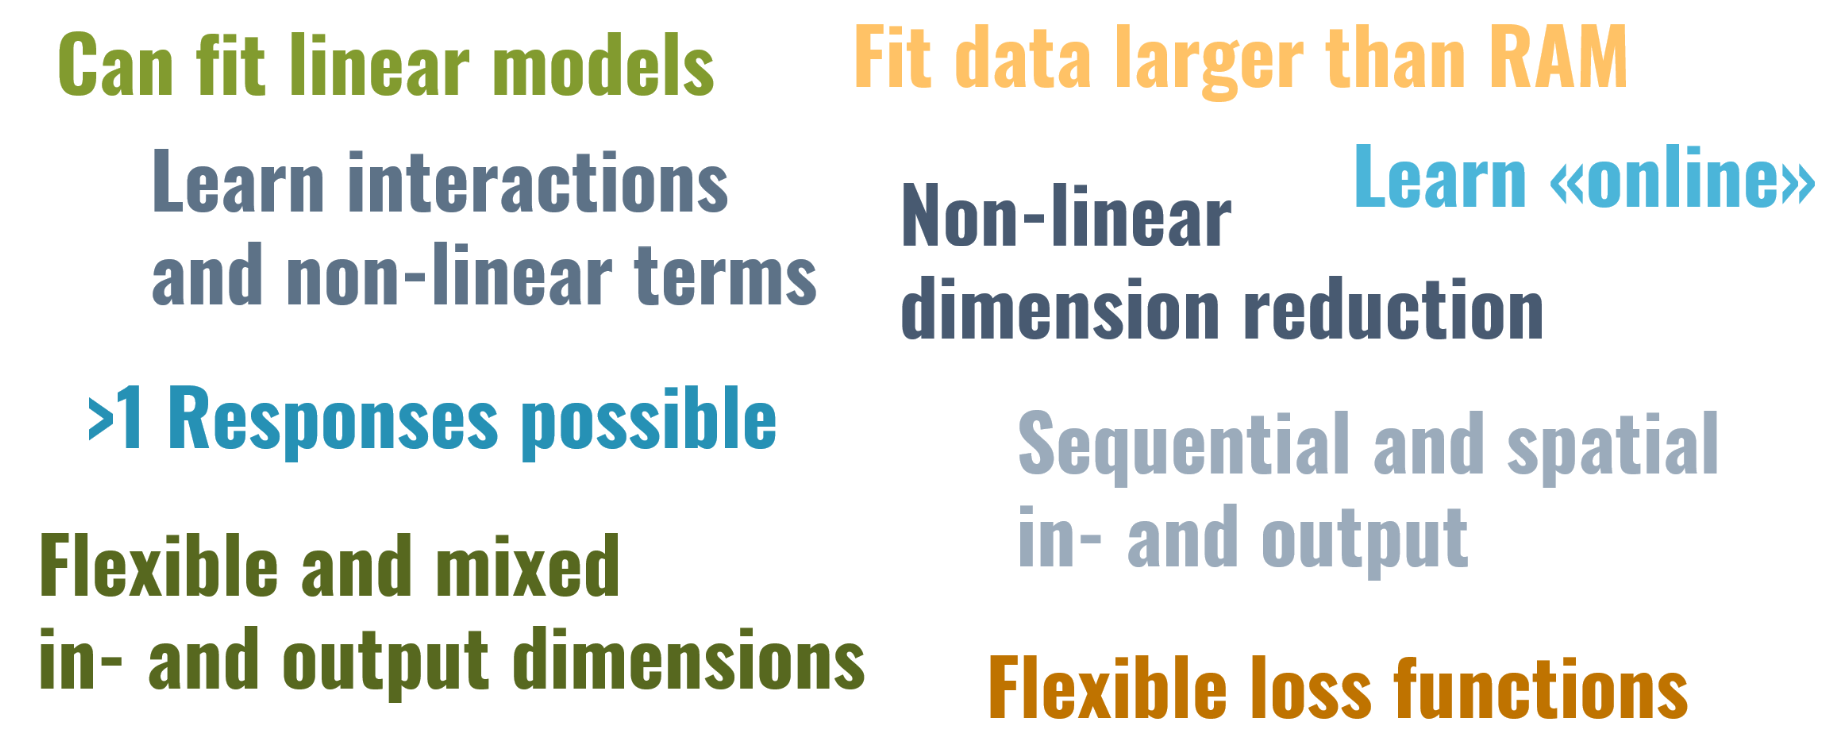
\includegraphics[width=0.9\textwidth]{pics/nn_knife.png}
	\end{figure}
\end{frame}

%=====================================================================
\subsection{Understanding Neural Nets}
%=====================================================================

\begin{frame}
	\frametitle{Understanding Neural Nets in three Steps}
	\begin{enumerate}
		\item Linear regression as neural net
		\item Hidden layers
		\item Activation functions
	\end{enumerate}
	
	\vfill
	
	Using \alert{diamonds} data
\end{frame}

\begin{frame}
	\frametitle{Step 1: Linear Regression as Neural Net}
	\begin{columns}
		\column{0.35\textwidth}
		\begin{itemize}
			\item $\E(\text{price})=\alpha+\beta \cdot \text{carat}$
			\item OLS 
			
			$\hat\alpha \approx -2256$, $\hat\beta \approx 7756$
			\item Represented as neural network graph
		\end{itemize}
		\column{0.65\textwidth}
		\begin{figure}
			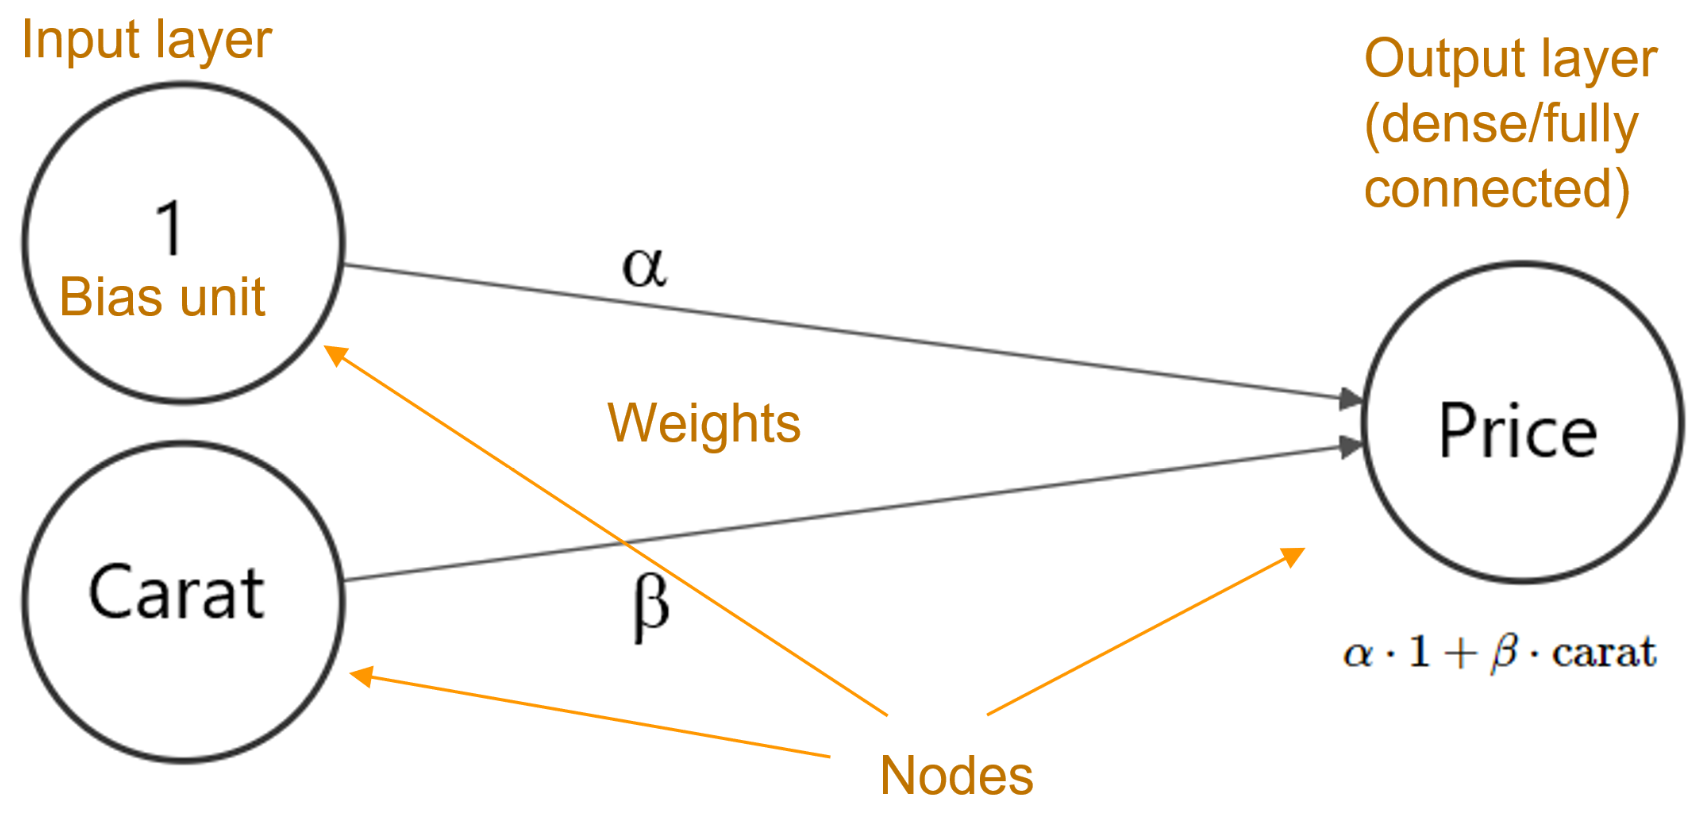
\includegraphics[width=0.9\textwidth]{pics/simple_nn.png}
		\end{figure}
	\end{columns}
	
	\vfill
	
	\begin{exampleblock}{\centering Example}
	\end{exampleblock}
\end{frame}

\begin{frame}
	\frametitle{The Optimization Algorithm}
	\begin{block}{Mini-batch gradient descent with backpropagation}
		Notation: Neural net $f_\beta$; its total loss on data $D$ and loss function $L$: 
		\vspace{-0.5em}
		$$
		Q(f_\beta, D) = \sum_{(y_i, \boldsymbol x_i) \in D} L(y_i, f_\beta(\boldsymbol x_i))
		$$
		\vspace{-1.2em}
		\begin{enumerate}
			\item Init: Randomly initialize parameter vector $\beta$ by $\hat \beta$
			\item Forward: Calculate $Q(f_{\hat\beta}, D_\text{batch})$ on \alert{batch}
			\item Backprop: Modify $\hat \beta$ to improve $Q(f_{\hat\beta}, D_\text{batch})$ 
			\begin{enumerate}
				\item Calculate partial derivatives $\nabla \hat \beta = \frac{\partial Q(f_\beta, D_\text{batch})}{\partial \beta}\mid_{\beta = \hat \beta}$ using backprop (=?)
				\item Gradient descent: Move slightly into right direction: $\hat \beta \leftarrow \hat \beta  - \lambda \cdot \nabla \hat \beta$
			\end{enumerate}
			\item Repeat Steps 2 and 3 until one \alert{epoch} is over
			\item Repeat Step 4 until some stopping criterion triggers
		\end{enumerate}
	\end{block}
	
	SGD? Local minima?
\end{frame}

\begin{frame}
	\frametitle{Step 2: Hidden Layers}
	\begin{columns}
		\column{0.33\textwidth}
		\begin{itemize}
			\item Add \alert{hidden layers} for more parameters 
			
			(= flexibility)
			\item Their nodes are latent/implicit variables
			\item Representational learning
			\item \small{\alert{Encoding}?}
			\item \small{\alert{Deep} neural net?}
		\end{itemize}
		\begin{example}
		\end{example}
		\column{0.67\textwidth}
		\begin{figure}
			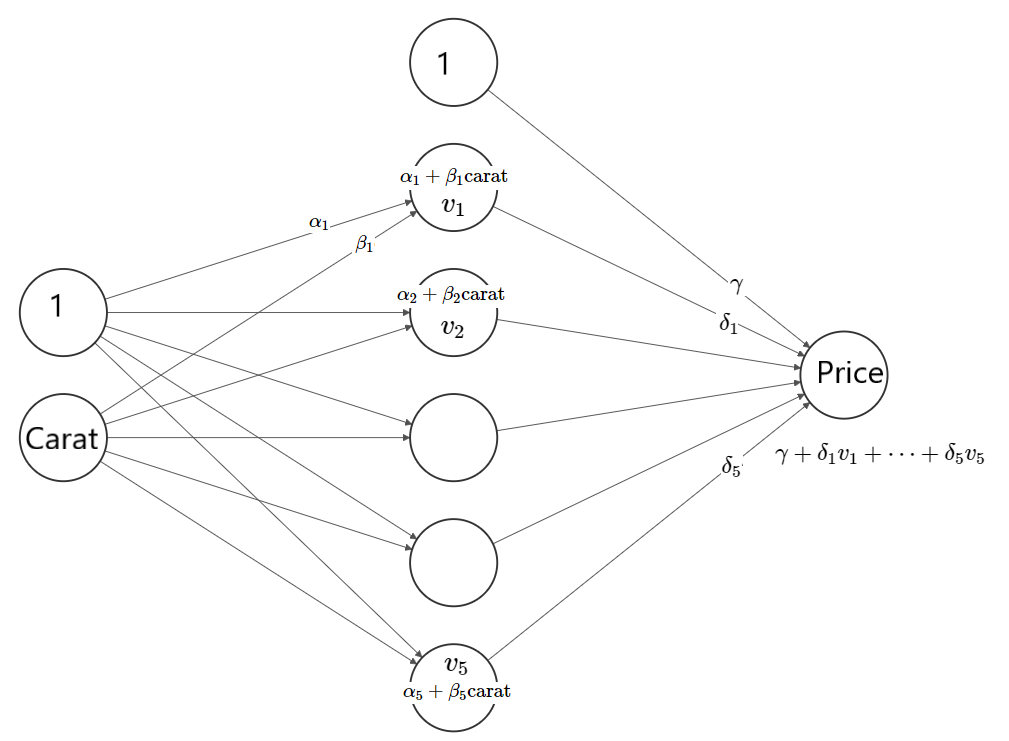
\includegraphics[width=0.98\textwidth]{../figs/nn_1_hidden.png}
		\end{figure}
	\end{columns}
\end{frame}

\begin{frame}
	\frametitle{Step 3: Activation Functions}
	Non-linear transformations $\sigma$ of node values necessary!
	\begin{columns}[onlytextwidth]
		\column{0.35\textwidth}
		\begin{itemize}
			\item tanh: $\sigma(x) = \frac{e^x - e^{-x}}{e^x + e^{-x}}$
			\item ReLU: $\sigma(x) = \text{max}(0, x)$
		\end{itemize}
		\begin{figure}
			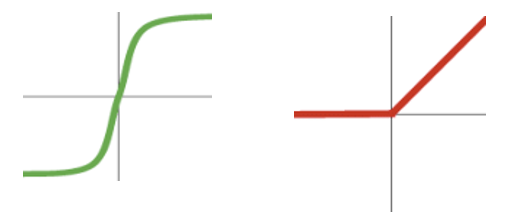
\includegraphics[width=0.8\textwidth]{pics/activation_functions.png}
		\end{figure}
		\begin{block}{Two purposes}
			\begin{itemize}
				\item Imply interactions and non-linear terms
				\item Inverse link as in GLMs
			\end{itemize}
		\end{block}
		\begin{example}
		\end{example}
		\column{0.65\textwidth}
		\begin{figure}
			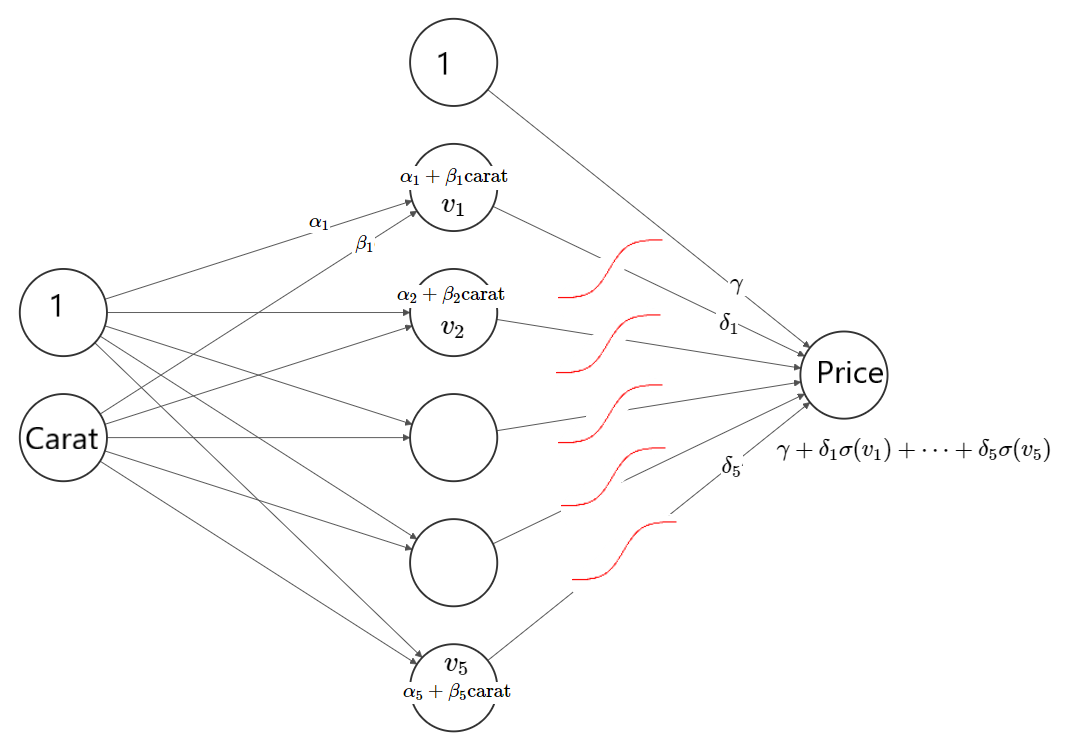
\includegraphics[width=0.98\textwidth]{../figs/nn_activation.png}
		\end{figure}
	\end{columns}
\end{frame}

%=====================================================================
\subsection{Practical Consideration}
%=====================================================================

\begin{frame}
	\frametitle{Practical Considerations}
	\begin{figure}
		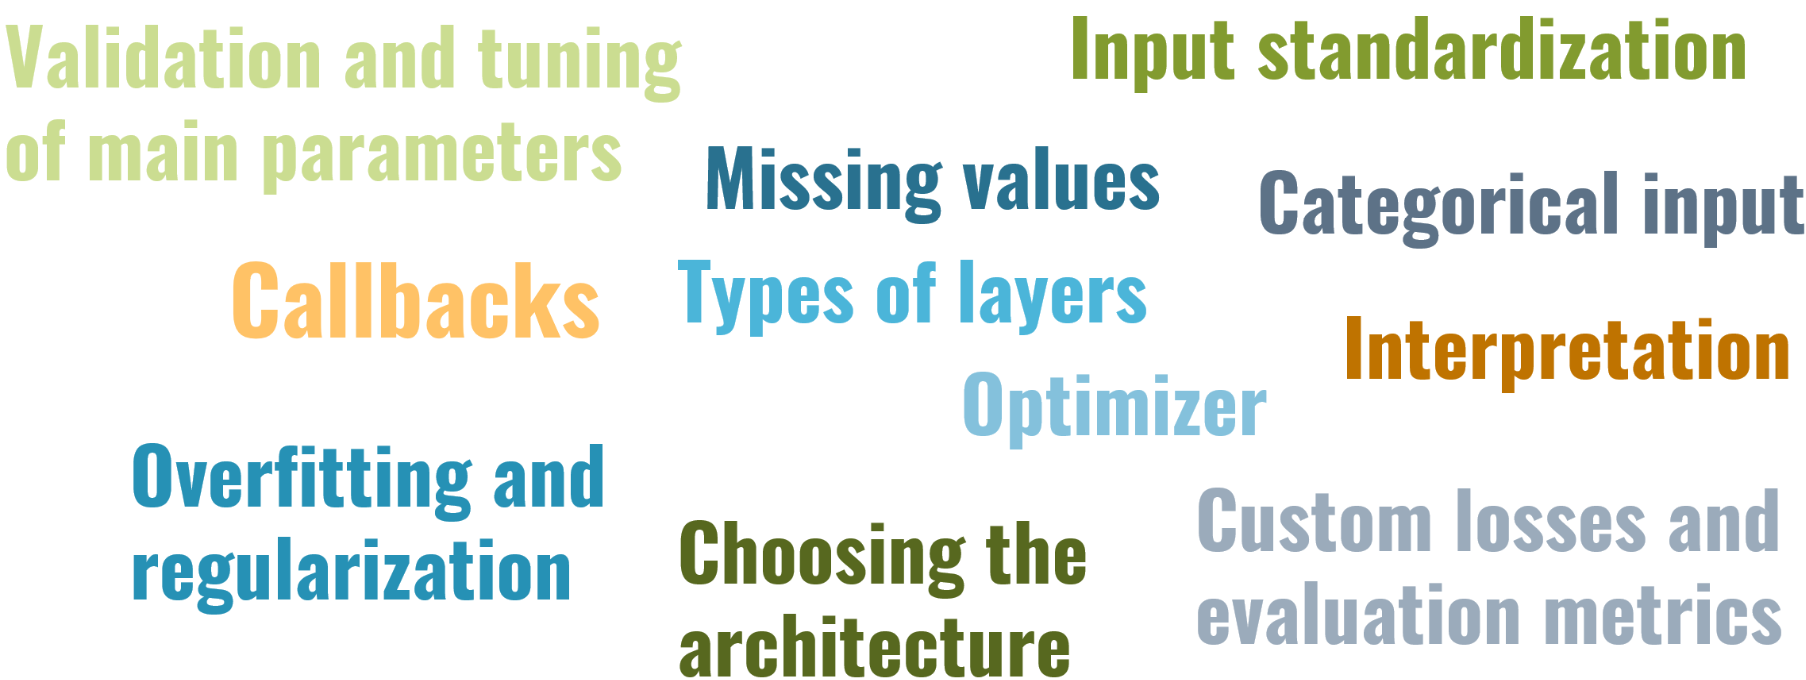
\includegraphics[width=0.9\textwidth]{pics/nn_practical.png}
	\end{figure}
\end{frame}

%=====================================================================
\subsection{Extended Examples}
%=====================================================================

\begin{frame}
	\frametitle{Example: Diamonds}
	\begin{figure}
		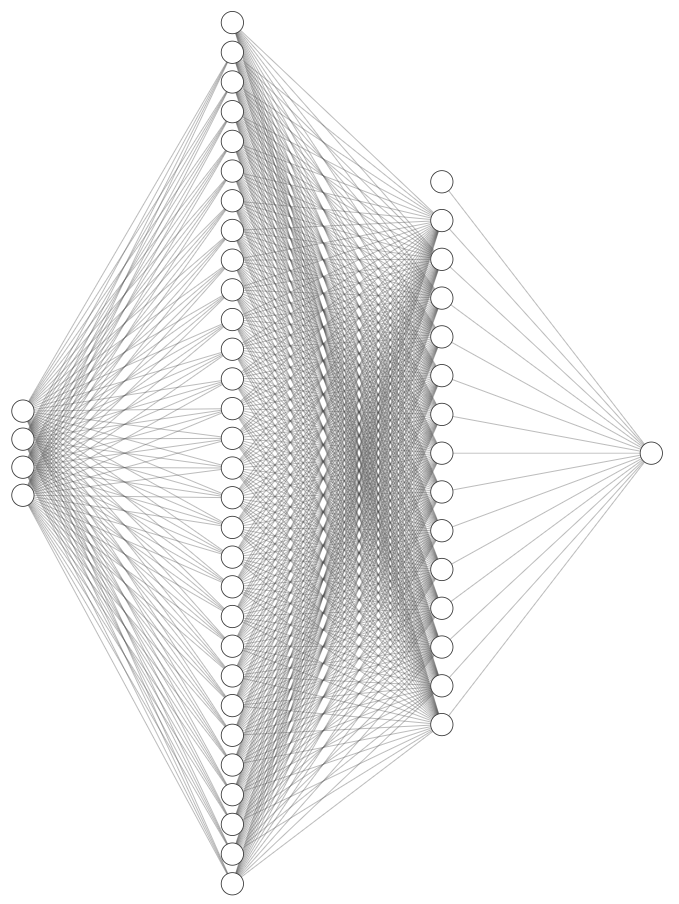
\includegraphics[width=0.6\textheight]{../figs/nn_2_hidden.png}
	\end{figure}
\end{frame}

\begin{frame}
	\frametitle{Excursion: Model-Agnostic Importance Measure}
	\alert{Permutation importance} of feature $X^{(j)}$, data $D$, and performance measure $S$:
	$$
	\text{PVI}(j, D) = S(\hat f, D^{(j)}) - S(\hat f, D)
	$$
	\vspace{-1.5em}
	\begin{itemize}
		\item $D^{(j)}$ is version of $D$ with randomly permuted values in $j$-th feature column
		\item Read: How much $S$ worsens after shuffling column $j$? 
		
		The larger, the more important. If 0, feature is unimportant
		\item Computationally cheap $\rightarrow$ repeat $m$ times
		\item Model is never refitted
		\item Training or test data?
	\end{itemize}
	
	\vfill
	
	\begin{example}
	\end{example}
\end{frame}

\begin{frame}
	\frametitle{Embeddings}
	Represent unordered categorical $X$ with $K$ levels by $m << K$ numeric features
	
	\vfill
	
	\begin{block}{Embedding layer}
		\begin{itemize}
			\item $X$ integer encoded
			\item Dummy matrix $\tilde X$ with $K$ columns
			\item Multiply $\tilde X$ with $(K \times m)$ matrix $\beta$
			\item Embedding matrix $\beta$ estimated like other parameters
			\item Trick: $\tilde X \beta$ is calculated via index slicing from $X$ and $\beta$
			
			$\rightarrow \tilde X$ is never materialized
		\end{itemize}
	\end{block}
	
	\vfill
	
	\begin{example}
		Taxi trips
	\end{example}
\end{frame}

%=====================================================================
\subsection{Excursion: Analysis Scheme X}
%=====================================================================

\begin{frame}
	\frametitle{Excursion: Analysis Scheme X}
	$T(Y)$: quantity of interest
	
	\vfill
	
	\begin{block}{Steps}
		\begin{enumerate}
			\item Calculate $T(Y)$ on the full data
			\item Calculate $T(Y)$ stratified by covariates $X^{(j)}$ $\rightarrow$ bivariate associations
			\item Accompany Step 2 by ML model $\rightarrow$ multivariate associations
			\begin{itemize}
				\item Study model performance
				\item Study variable importance $\rightarrow$ sort results of Step 2
				\item Study PDP (or similar) for each $X^{(j)}$ and compare with Step 2
			\end{itemize}
		\end{enumerate}
	\end{block}
	
	\vfill
	
	\begin{example}
	\end{example}
\end{frame}

%=====================================================================
\subsection{Outro}
%=====================================================================

\begin{frame}
	\frametitle{Comparison of ML Algorithms}
	\begin{figure}
		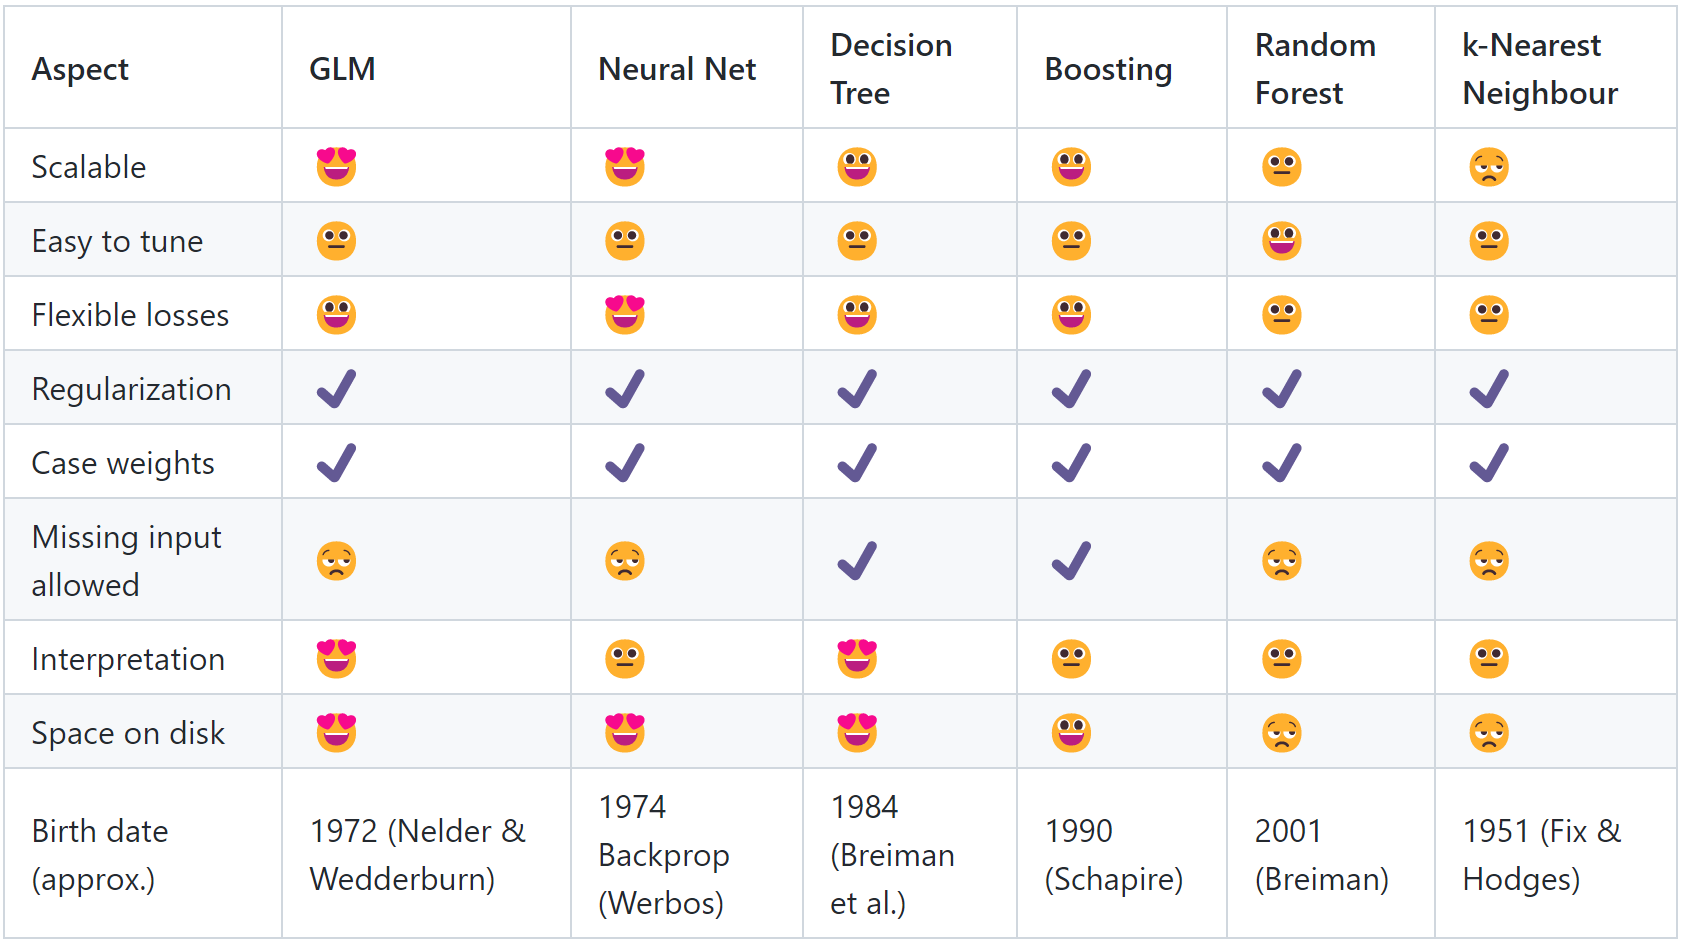
\includegraphics[width=0.9\textwidth]{pics/algorithms.png}
	\end{figure}
\end{frame}